

\chapter{Choix et justifications}

\section{Choix des capteurs}
\vspace{1.5cm}
Après avoir réalisé l'état de l'art pour notre système de surveillance d'une ruche, nous nous sommes ensuite intéressés aux capteurs que nous allons employer.\\

\textbf{Capteur de température}\\

Nous avons choisis un capteur de température identique pour recueillir la température interne et externe de la ruche.
Il s'agit d'une thermistance NTC boitier Goutte Radial 1000 ohms sortie fil de cuivre émaillé 1 pc(s). Ce dernier possède une gamme de mesure comprise entre -40 C et 100 C ce qui correspond bien aux exigences discutées avec le client (Voir tableau des exigences). Le capteur placé à l'extérieur nous renseignera sur les conditions météorologique et expliquer une éventuelle diminution de la production de miel par exemple. Celui placé à l'intérieur nous donnera une idée de l'isolation de la ruche en hiver et de sa ventilation en été.\\  

\textbf{Capteur d'humidité}\\

On a choisit d'inclure ce capteur dans notre système compte tenu des résultats de l'état de l'art. Néanmoins, après discussion avec le client, cette option n'est pas primordiale pour un apiculteur mais elle sera tout de même rajoutée au tableau de bord du serveur.\\

\textbf{Capteur de pression}\\

Les capteurs de pression vont nous permettre de récupérer le poids de ruche et surtout celui des hausses pour avertir l'apiculteur de la quantité de miel produite. Pour se faire, le projet Bzzz développé par le Fablab de Lannion a prévu d'utiliser deux sachets de "Pompote" remplis d'eau sucrée pour éviter les variations de pression atmosphérique, le gel et l'évaporation. Cependant, après avoir pris conscience de l'importance de la localisation de la grappe, nous avons pensé installer deux capteurs de pression par cadre (au niveau de chaque extrémité) soit 20 au total mais cette solution s'est avérée être difficile à mettre en place à cause de la surface sur laquelle repose les cadres (simple lamelle en métal). Après discussion avec le client, nous avons finalement opté pour la confection d'un cadre en bois aux même dimensions de la ruche dans lequel se trouverons les capteurs de pression. L'utilisateur décidera de l'endroit où le placer en fonction des données qu'il veut récupérer. 
On pourra aussi utiliser ce capteur pour détecter l'ouverture du couvercle à cause du vent.\\

\textbf{Tilt sensor}\\

Ce capteur permet de savoir si la ruche a reçu un choc ou si elle a été déplacé. Il renvoi une information binaire qui pourra être couplée avec les données de la carte GPS et ainsi avertir l'apiculteur en cas de détérioration, renversement ou vol de la ruche. Ce dernier évènement étant de plus en plus fréquent.
Nous avons choisit le TikerKit Tilt Sensor \ref{fig:tiltSensor}.\\

\begin{figure}[h]
\centering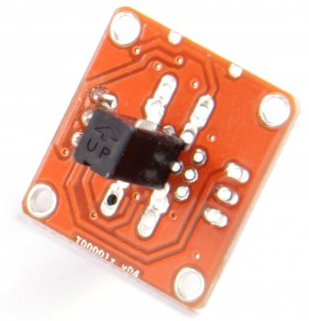
\includegraphics[scale=0.5]{tiltSensor.png}
\caption{\label{fig:tiltSensor} TikerKit Tilt Sensor}
\end{figure} 
     

\textbf{Microphone}\\

L'utilisation d'un microphone s'est imposée comme une nécessité dans la surveillance d'une ruche car il permet de recueillir des données pouvant avertir l'apiculteur sur plusieurs types d'évènements. En effet, grâce à ce dernier, on pourra détecter la présence d'abeilles dans la ruche notamment en hiver et éventuellement recueillir la source du bourdonnement et ainsi localiser la grappe approximativement. On pourra aussi détecter les prémisses d'un essaimage en percevant le champs d'une raine caractéristique de ce type d'évènement. Cette information pourra ensuite être couplée avec les données des capteurs de pression et confirmer l'essaimage en cours si le poids chute brutalement. 
Nous avons choisit le Capsule micro pour CI 2 V/DC sensibilité 44 dB (à 3 dB près) sur la plage 100 - 10000 Hz. 

\section{Choix de la carte Arduino}
\vspace{1.5cm}

Compte tenu du fait que nous avions besoin d'un nombre d'entrées assez élevé (au moins 20) ainsi que d'un temps ADC supérieur ou égal à 5kHz. Nous avons alors sélectionné quatre cartes, que nous avons ensuite comparées. Ces résultats sont regroupés dans la Figure\ref{fig:choixardui}.

\begin{figure}[h]
\centering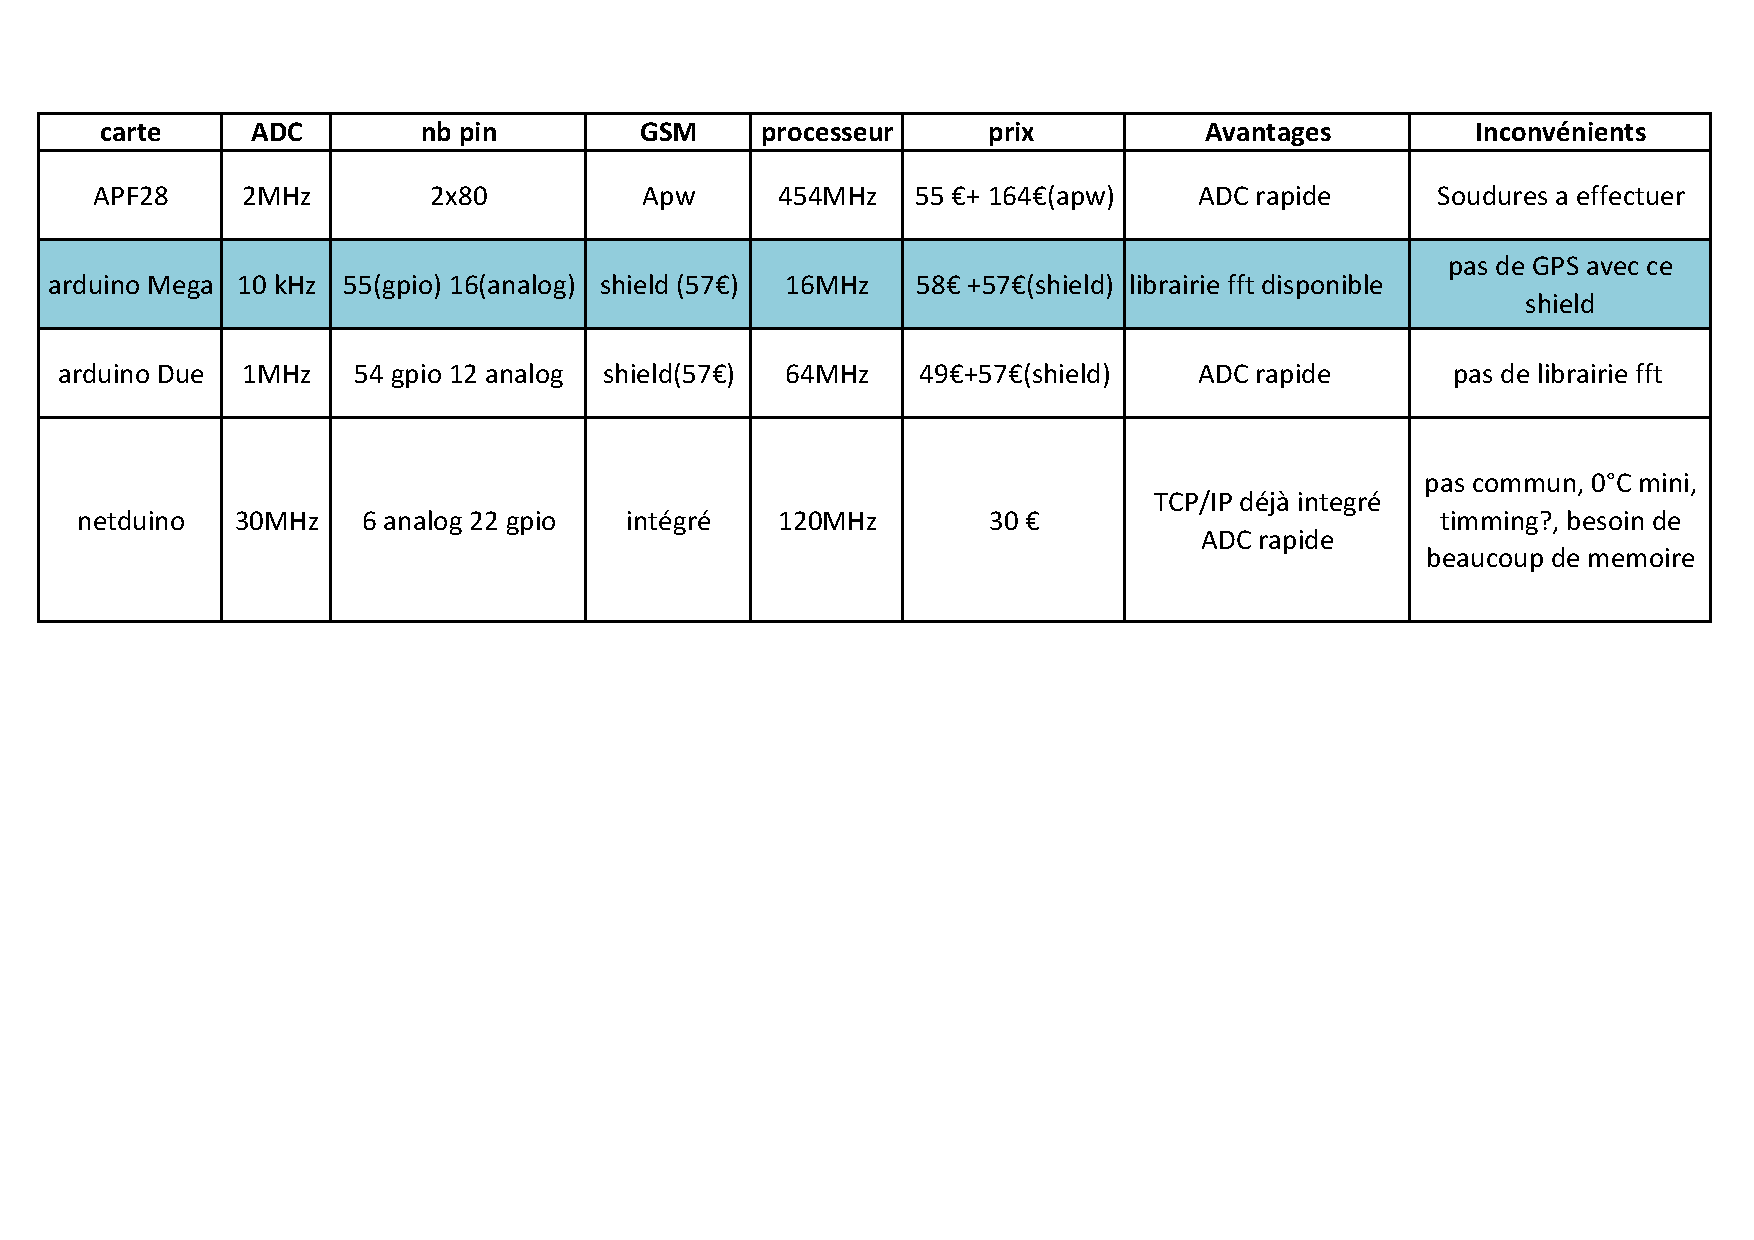
\includegraphics[trim=1cm 11cm 1cm 1cm,scale=0.5]{choixArduino.pdf}
\caption{\label{fig:choixardui} Tableau comparatif des cartes Arduino et équivalents}
\end{figure} 

Nous avons opté pour une carte Arduino Mega 2560, Figure \ref{fig:arduino}, compte tenu de l'existence de nombreuses librairies, notamment pour réaliser une fft, et du prix raisonnable. La carte netduino paraissait également très intéressante, car elle ne nécessite pas de shield supplémentaire pour accéder à internet et était trois fois moins chère que les autres. Cependant, comme ce système est peu utilisé, il sera difficile de trouver de la documentation sur internet. Enfin ce système utilise beaucoup de mémoire pour son fonctionnement, limitant ainsi la capacité de stockage. Nous ne pouvions donc pas envisager cette solution et nous avons donc choisi la carte classique Arduino Mega 2560.


\begin{figure}[h]
\centering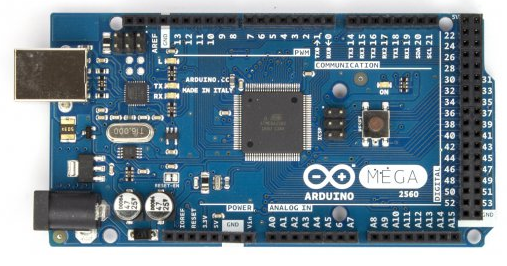
\includegraphics[scale=0.5]{arduino.png}
\caption{\label{fig:arduino} Carte Arduino Mega 2560}
\end{figure} 

\section{Choix de la solution technique}
\vspace{1.5cm}

Nous avons décidé d'opter pour une solution technique simple à déplacer et qui peut ainsi s'adapter à l'utilisateur.
En effet,suite à nos échanges avec notre client, monsieur Singhoff, nous avons remarqué que selon la période de l'année les besoins de l'apiculteur ne sont pas les mêmes. En hivers il veut des informations sur le corps de la ruche alors qu'en été il s'intéresse plus aux hausses qu'il ajoute. Ainsi dans un soucis d'efficacité et de maniabilité, nous voulons intégrer nos capteurs à un cadre en bois que l'apiculteur placera selon ses besoins. Il disposera le cadre sous la partie de la ruche qu'il veut surveiller. Ainsi en hiver, le cadre de mesure sera normalement placé sous la ruche, Figure \ref{fig:rucheBas}, pour vérifier l'activité et les réserves disponibles pour les abeilles. En été, le cadre de mesure sera placé sous une des hausses,Figure \ref{fig:rucheHaut}, logiquement la dernière pour suivre la miellée.
\begin{figure}[h]

\begin{minipage}[c]{.46\linewidth}
     \begin{center}
             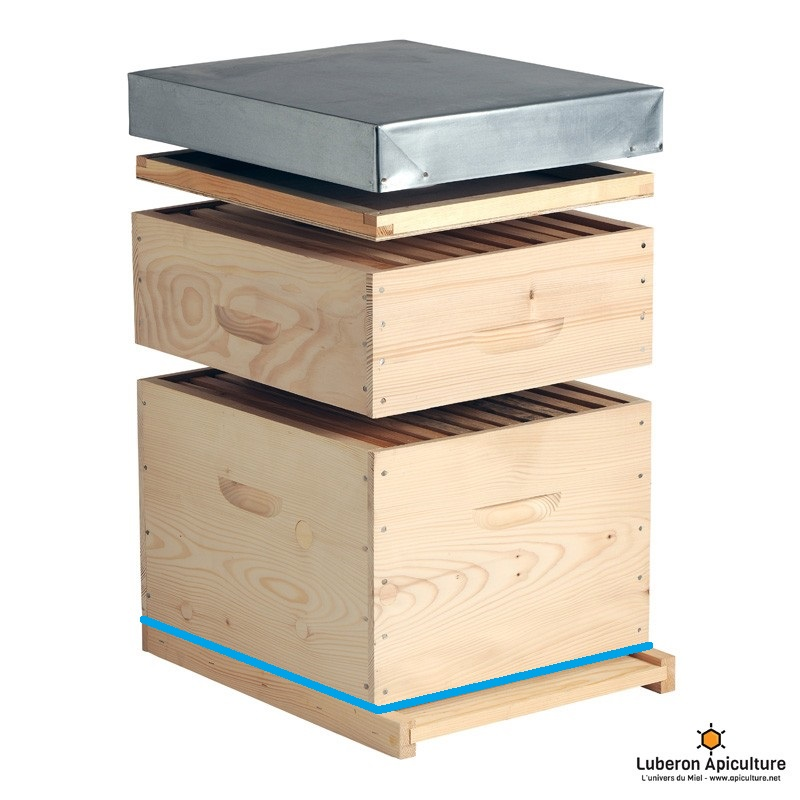
\includegraphics[scale=0.4]{cadreBas.jpg}
             \caption{\label{fig:rucheBas} Position standard du cadre de mesure en hiver}
         \end{center}
   \end{minipage} \hfill
   \begin{minipage}[c]{.46\linewidth}
    \begin{center}
            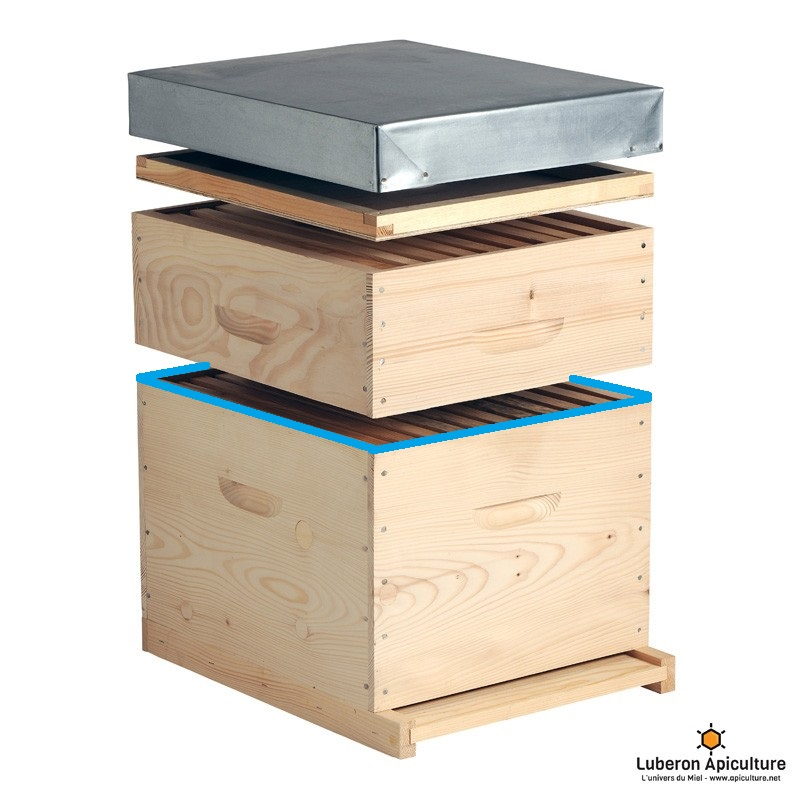
\includegraphics[scale=0.4]{cadreHaut.jpg}
            \caption{\label{fig:rucheBas} Position standard du cadre de mesure en été}
        \end{center}
 \end{minipage}
 \end{figure}

\chapter{Résultats et analyses}

analyse des tests et des performances
analyse des échecs, des décalages et des retards
Que reste-t-il à faire ? Comment ?


\chapter{Conclusion}
